% Provenance (never printed): see sources/outline_sources.md (Year 3:
% ocean dynamics: the Ekman layer derived, the Sverdrup balance, western
% intensification, the abyssal circulation, ocean tides).
% Brief: sources/book5/BRIEFS.md, ch. 21. Curves from
% figdata/bachelor-3/wind_driven_gyre.py and tides.py. Exercise and problem
% values in the Book 5 scratch calculator calc/ch21.py. The basins, winds
% and stations of the exercises and the problem are invented.
\chapter{Oceaandynamica}\label{ch:b3:ocean-dynamics}

Door de Straat van Florida voert de Golfstroom ongeveer
\qty{32}{\sverdrup} water noordwaarts, en de stroom neemt toe terwijl hij
langs de kust naar het noorden loopt, tot ongeveer \qty{150}{\sverdrup} bij \ang{40}~NB. Aan de andere kant van dezelfde oceaan, voor Portugal en
Noord-Afrika stroomt niets dat er ook maar op lijkt naar het zuiden: het water dat de Golfstroom
naar het noorden brengt keert terug naar de evenaar als een trage, brede drift over duizenden
kilometers open zee. Elk oceaanbekken op het Noordelijk Halfrond heeft
dezelfde scheve vorm, met de snelle stroom aan de westkant. De
asymmetrie volgt uit de wind, uit de wrijving van de zee en uit één
feit over de Aarde: de Coriolisparameter neemt toe naar de pool toe.
% ledger: rapid:transports (31.7 Sv, rounded), stewart:north-atlantic

\begin{recall}
De getijkracht van de Maan en de Zon, springtij en doodtij, staan in de
natuurkundeboeken. De windschuifspanning, de Ekmanlaag, het Ekmantransport en
de Ekmanspiraal, opwelling en neerwaartse stroming, de gyres, de westelijke
randstromen, de sverdrup ($\qty{1}{\sverdrup} =
\qty{e6}{m^3/s}$), de meridionale omkeercirculatie en de
vorming van diep water staan in Boek~3, in het hoofdstuk over de
oceaancirculatie; daar wordt de windschuifspanning geschreven als $\vec T$, hier
$\vec\tau$. De Coriolisparameter, het $\beta$-vlak, de Rossbystraal en
het geostrofisch evenwicht staan in Hoofdstuk~\ref{ch:b3:gfd-foundations};
vorticiteit en \omterm{def:b3:atmospheric-dynamics:pv}{potentiële vorticiteit} in Hoofdstuk~\ref{ch:b3:atmospheric-dynamics}.
\end{recall}

\section{De Ekmanlaag afgeleid}\label{sec:b3:ocean-dynamics:ekman}

In Boek~3 werd het Ekmantransport gevonden uit een evenwicht van krachten
over de hele laag, en de spiraal van snelheden erin werd gegeven. Bij een
turbulente wrijving met constante wervelviscositeit $A_z$ volgt de spiraal
uit de vergelijkingen in enkele regels. Schrijf de horizontale snelheid als een
complex getal, $W = u + \mathrm iv$, en de windschuifspanning als $\tau =
\tau_x + \mathrm i\tau_y$; vermenigvuldigen met $-\mathrm i$ draait een vector
over \ang{90} met de klok mee, naar rechts gezien van boven.

\begin{theorem}[Snelheidsprofiel van een stationaire, door wind aangedreven oppervlaktelaag]\label{thm:b3:ocean-dynamics:ekman}
In een stationaire, horizontaal uniforme oceaan van grote diepte en constante dichtheid
$\rho$, met een constante verticale wervelviscositeit $A_z$ en de Coriolisparameter
$f > 0$, wordt de stroming die door een windschuifspanning $\tau$ wordt aangedreven
\[
W(z) = W_0\,\mathrm e^{(1+\mathrm i)z/\delta},\qquad
W_0 = \frac{\tau}{\rho\sqrt{fA_z}}\,\mathrm e^{-\mathrm i\pi/4},\qquad
\delta = \sqrt{\frac{2A_z}{f}} ,
\]
voor $z \le 0$. De oppervlaktestroom wordt over \ang{45} naar rechts van de
spanning gedraaid; met de diepte draait hij verder naar rechts en neemt af als $\mathrm
e^{z/\delta}$; het totale transport $\int_{-\infty}^0 W\,\mathrm dz =
-\mathrm i\tau/(\rho f)$ staat loodrecht op de rechterkant van de spanning.
\end{theorem}

\begin{proof}
Buiten de kusten is er in de laag geen horizontale drukgradiënt,
en de Corioliskracht houdt de wrijving in evenwicht: $-fv = A_z u''$ en $fu =
A_z v''$, waarbij de accenten afgeleiden naar $z$ zijn. Vermenigvuldig de tweede
vergelijking met $\mathrm i$ en tel op; dat geeft $A_zW'' = \mathrm ifW$. De oplossingen zijn
$\mathrm e^{\pm(1+\mathrm i)z/\delta}$, want $(1+\mathrm i)^2/\delta^2 =
2\mathrm i/\delta^2 = \mathrm if/A_z$; alleen het plusteken blijft begrensd voor
$z \to -\infty$. Aan het oppervlak wordt de spanning door de wrijving gedragen,
$\rho A_zW'(0) = \tau$, dus $W_0 = \tau\delta/(\rho A_z(1+\mathrm i))$.
Omdat $\delta/(\sqrt2 A_z) = 1/\sqrt{fA_z}$ en $1/(1+\mathrm i) = \mathrm
e^{-\mathrm i\pi/4}/\sqrt2$, is dit de gegeven $W_0$. De factor
$\mathrm e^{\mathrm iz/\delta}$ draait met de klok mee naarmate $z$ afneemt. Ten slotte
$\int_{-\infty}^0 W\,\mathrm dz = W_0\delta/(1+\mathrm i) =
\tau\delta^2/(\rho A_z(1+\mathrm i)^2) = \tau\delta^2/(2\mathrm i\rho A_z)
= -\mathrm i\tau/(\rho f)$.
\end{proof}

De stelling herleidt beide resultaten van Boek~3: Ekmans oppervlaktestroom
onder \ang{45} en het transport $\tau/(\rho f)$, loodrecht op de spanning en
onafhankelijk van $A_z$, dat nooit goed bekend is. Op de
diepte $\pi\delta$ stroomt de stroming tegen de oppervlaktestroom in, verminderd
met $\mathrm e^{-\pi}$, tot \qty{4}{\percent}.

\begin{definition}[Ekmandiepte; Ekmanpompen]\label{def:b3:ocean-dynamics:ekman-pumping}
De \emph{Ekmandiepte}\index{Ekmandiepte} is $D_E = \pi\delta =
\pi\sqrt{2A_z/f}$, de diepte waarop de stroming van de Ekmanspiraal
tegen de oppervlaktestroom in stroomt; zij meet de dikte van de
Ekmanlaag. \emph{Ekmanpompen}\index{Ekmanpompen} is de verticale
snelheid $w_E$ aan de onderkant van de Ekmanlaag, veroorzaakt door de convergentie of
divergentie van het Ekmantransport: neerwaarts waar de transporten
convergeren, opwaarts, soms Ekmanzuiging genoemd, waar ze divergeren.
\end{definition}

\begin{proposition}[Ekmanpompen]\label{prop:b3:ocean-dynamics:pumping}
Met de verticale snelheid nul aan het zeeoppervlak is het \omterm{def:b3:ocean-dynamics:ekman-pumping}{Ekmanpompen}
\[
w_E = \operatorname{curl}_z\frac{\vec\tau}{\rho f}
= \frac{1}{\rho f}\Big(\frac{\partial\tau_y}{\partial x} -
\frac{\partial\tau_x}{\partial y}\Big) + \frac{\beta\tau_x}{\rho f^2} ,
\]
opwaarts positief.
\end{proposition}

\begin{proof}
Het volumetransport van de laag is $(U_E, V_E) = (\tau_y,
-\tau_x)/(\rho f)$, de stelling in componenten geschreven. Integreer de
continuïteitsvergelijking $\partial w/\partial z = -(\partial u/\partial x +
\partial v/\partial y)$ door de laag heen; dan geldt $w(0) - w_E = -(\partial
U_E/\partial x + \partial V_E/\partial y)$, dus $w_E = \partial_x(\tau_y/\rho
f) - \partial_y(\tau_x/\rho f)$. Uitwerken met $\mathrm df/\mathrm dy =
\beta$ geeft de tweede vorm.
\end{proof}

Een wind die boven de zee cyclonaal draait, met een positieve rotatie, trekt
water van onder de laag omhoog; een anticyclonale wind duwt het omlaag. In de subtropische oceanen
waaien de passaten van het oosten aan de
equatorzijde, de westenwinden van het westen aan de poolzijde. Hun Ekmantransporten,
noord onder de passaten en zuid onder de westenwinden,
convergeren ertussen: het oppervlaktewater hoopt zich op en wordt omlaag gepompt, zoals
in de figuur hieronder. Langs een kust waar de
wind waait met de kust links van zich (op het Noordelijk Halfrond), het
transport gaat van de kust weg en de kustopwelling uit Boek~3 is
Ekmanzuiging, geconcentreerd tegen een wand.

\begin{omfigure}
\centering
\begin{tikzpicture}[>=stealth, font=\small, x=1.1cm, y=1cm]
\fill[omThm!7] (-5,0) rectangle (5,-3.6);
\draw[thick] (-5,0) -- (5,0);
\draw[black!45, densely dashed] (-5,-0.9) -- (5,-0.9);
\node[font=\scriptsize, black!60, anchor=north east, inner sep=1pt] at (4.95,-0.95) {Ekmanlaag};
% winds: west is out of the page, east into the page
\foreach \x in {-4.2,-3.4,-2.6} {\draw (\x,0.55) circle (0.13); \fill (\x,0.55) circle (0.04);}
\foreach \x in {2.6,3.4,4.2} {\draw (\x,0.55) circle (0.13);
  \draw (\x-0.09,0.46) -- (\x+0.09,0.64); \draw (\x-0.09,0.64) -- (\x+0.09,0.46);}
\node[above] at (-3.4,0.75) {passaten, uit het oosten};
\node[above] at (3.4,0.75) {westenwinden, uit het westen};
% Ekman transports converge
\draw[->, omDef, very thick] (-4.5,-0.45) -- (-1.2,-0.45);
\draw[->, omDef, very thick] (4.5,-0.45) -- (1.2,-0.45);
\node[omDef, font=\scriptsize, fill=omThm!7, inner sep=1pt] at (-2.85,-0.72) {Ekmantransport};
% pumping
\foreach \x in {-0.6,0,0.6} \draw[->, omThm, thick] (\x,-0.55) -- (\x,-1.55);
\node[omThm, font=\scriptsize, anchor=west] at (0.75,-1.25) {$w_E < 0$};
% squashed column and Sverdrup flow
\draw[thick, black!70] (-0.62,-1.75) rectangle (0.62,-3.1);
\node[font=\scriptsize, black!70, align=center] at (0,-2.42) {kolom\\samengedrukt};
\draw[->, omMeth, very thick] (-0.75,-2.42) -- (-3.2,-2.42);
\node[omMeth, font=\scriptsize, align=center, above] at (-2.6,-2.40) {Sverdrupstroming,\\richting de evenaar};
\draw[black!45, densely dashed] (-5,-3.3) -- (5,-3.3);
\node[font=\scriptsize, black!60, anchor=south east, inner sep=1pt] at (4.95,-3.28) {basis van de windgedreven stroming};
\node[below, font=\scriptsize] at (-5,-3.6) {zuid};
\node[below, font=\scriptsize] at (5,-3.6) {noord};
\end{tikzpicture}

\par\smallskip{\small Een noord--zuid-doorsnede door een subtropische gyre
van het Noordelijk Halfrond, oostwaarts de pagina in. De Ekmantransporten onder
de passaten en de westenwinden convergeren, het water wordt omlaag gepompt, en de
kolommen eronder, samengedrukt, bewegen richting de evenaar, waar $f$ kleiner is,
om hun \omterm{def:b3:atmospheric-dynamics:pv}{potentiële vorticiteit} te behouden.}\label{fig:b3:ocean-dynamics:pumping}
\end{omfigure}

\section{De Sverdrupbalans}\label{sec:b3:ocean-dynamics:sverdrup}

Onder de Ekmanlaag is de oceaan geostrofisch. Een waterkolom die
door \omterm{def:b3:ocean-dynamics:ekman-pumping}{Ekmanpompen} wordt samengedrukt, moet om haar \omterm{def:b3:atmospheric-dynamics:pv}{potentiële vorticiteit} $f/h$ te behouden,
naar een plek waar $f$ kleiner is: richting de evenaar. In 1947 werkte H.~U.~Sverdrup
het argument kwantitatief uit voor de hele diepte van de windgedreven stroming.
% ledger: stewart:ekman-layer (Sverdrup 1947)

\begin{theorem}[Sverdrupbalans]\label{thm:b3:ocean-dynamics:sverdrup}
In een stationaire oceaan waarin de niet-lineaire termen en de laterale wrijving
verwaarloosbaar zijn, is het inwendige geostrofisch onder de Ekmanlaag, en de
verticale snelheid op een diepte $-H$ nul is, het totale noordwaartse volumetransport
per breedte-eenheid van de windgedreven stroming voldoet aan de \emph{Sverdrup
balans}\index{Sverdrupbalans}
\[
\beta V = \frac{1}{\rho}\operatorname{curl}_z\vec\tau
= \frac{1}{\rho}\Big(\frac{\partial\tau_y}{\partial x} -
\frac{\partial\tau_x}{\partial y}\Big) .
\]
\end{theorem}

\begin{proof}
In het geostrofische inwendige $fv_g = \rho^{-1}\partial p/\partial x$ en
$fu_g = -\rho^{-1}\partial p/\partial y$. Dus $\partial_x(fu_g) +
\partial_y(fv_g) = 0$, dat wil zeggen $f(\partial_xu_g + \partial_yv_g) + \beta
v_g = 0$, en met continuïteit geldt $\beta v_g = f\,\partial w/\partial z$.
Integreer van $-H$, waar $w = 0$, tot aan de onderkant van de Ekmanlaag,
waar $w = w_E$, dat geeft $\beta V_g = fw_E$. Volgens
\cref{prop:b3:ocean-dynamics:pumping}, $fw_E = \rho^{-1}\operatorname{curl}_z
\vec\tau + \beta\tau_x/(\rho f)$. Bij optellen van het Ekmantransport $V_E =
-\tau_x/(\rho f)$, vermenigvuldigd met $\beta$, heft de laatste term op:
$\beta(V_g + V_E) = \rho^{-1}\operatorname{curl}_z\vec\tau$.
\end{proof}

De balans is opmerkelijk door wat ze niet nodig heeft: noch de diepte van
de stroming, noch haar verticale structuur, noch de wervelviscositeit, alleen de
rotatie van de wind en $\beta$. Sverdrup leidde haar af uit de bewegingsvergelijkingen
geïntegreerd tot op een diepte zonder beweging, en toetste haar aan de
hydrografische doorsneden van de onderzoeksschepen \emph{Carnegie} en
\emph{Bushnell} in de oostelijke tropische Stille Oceaan, tussen \ang{34} NB en
\ang{10} ZB, met een diepte zonder beweging op \qty{1000}{m}: de transporten
berekend uit de wind kwamen overeen met die uit het dichtheidsveld, zelfs
waar de stromen tegen de wind in liepen. Latere studies met betere winden
vonden de beste overeenstemming bij een diepte zonder beweging nabij \qty{500}{m}, en
metingen van de gemiddelde spanning in de equatoriale Stille Oceaan in 1999 vonden de
stroming daar in \omterm{thm:b3:ocean-dynamics:sverdrup}{Sverdrupbalans}. Of de balans overal opgaat is
moeilijker aan te tonen dan aan te nemen: bijna elke theorie van de oceaancirculatie
gaat ervan uit.
% ledger: stewart:sverdrup

Beschouw het verzonnen bekken uit het probleem van dit hoofdstuk: tussen \ang{20} en
\ang{50} NB, \qty{6000}{km} breed, onder een zonale spanning $\tau_x =
-\tau_0\cos(\pi(\varphi - \ang{20})/\ang{30})$ met $\tau_0 =
\qty{0.1}{Pa}$, oostelijk bij \ang{20} NB, westelijk bij \ang{50} NB, nul bij
\ang{35} NB. Over bijna het hele bekken is de spanningsrotatie negatief: het
water wordt omlaag gepompt, met ongeveer \qty{35}{m} per jaar bij \ang{35} NB, en de
inwendige stroming gaat naar het zuiden, \qty{4.9}{m^2/s} per meter breedte bij \ang{35} NB,
\qty{29.4}{\sverdrup} over het hele bekken. Berekend uit de waargenomen winden,
het Sverdruptransport van de subtropische gyre van de Noord-Atlantische Oceaan bereikt
ongeveer \qty{30}{\sverdrup} nabij \ang{28} NB.
% ledger: stewart:north-atlantic (computed in figdata/bachelor-3/wind_driven_gyre.py)

\begin{omfigure}
\begin{tikzpicture}
\begin{groupplot}[group style={group size=3 by 1, horizontal sep=0.45cm, yticklabels at=edge left},
  width=0.37\linewidth, height=0.46\linewidth, ymin=20, ymax=50, ytick={20,25,30,35,40,45,50},
  tick label style={font=\scriptsize}, label style={font=\small}, title style={font=\small}]
\nextgroupplot[xlabel={$\tau_x$ (\unit{Pa})}, ylabel={breedtegraad (\unit{\degree} NB)},
  xmin=-0.12, xmax=0.12, xtick={-0.1,0,0.1}, title={windschuifspanning},
  scaled x ticks=false, xticklabel style={/pgf/number format/fixed}]
% computed in figdata/bachelor-3/wind_driven_gyre.py
\addplot[black!50, thin] coordinates {(0,20) (0,50)};
\addplot[omThm, thick] table[x=tau, y=lat] {figdata/out/bachelor-3-wind_driven_gyre-merid.dat};
\nextgroupplot[xlabel={$w_E$ (\unit{m/yr})}, xmin=-45, xmax=12, xtick={-40,-20,0},
  title={Ekmanpompen}]
\addplot[black!50, thin] coordinates {(0,20) (0,50)};
\addplot[omDef, thick] table[x=wE, y=lat] {figdata/out/bachelor-3-wind_driven_gyre-merid.dat};
\nextgroupplot[xlabel={transport (\unit{\sverdrup})}, xmin=-32, xmax=10, xtick={-30,-20,-10,0,10},
  title={Sverdrup}]
\addplot[black!50, thin] coordinates {(0,20) (0,50)};
\addplot[omMeth, thick] table[x=Vtot, y=lat] {figdata/out/bachelor-3-wind_driven_gyre-merid.dat};
\end{groupplot}
\end{tikzpicture}

\par\smallskip{\small Het verzonnen bekken van het probleem, \ang{20} tot
\ang{50} NB en \qty{6000}{km} breed. Links de zonale windschuifspanning, naar het oosten
positief. Midden de \omterm{def:b3:ocean-dynamics:ekman-pumping}{Ekmanpompen}, omhoog positief: het water wordt omlaag gedrukt
ten zuiden van \ang{47} NB, het sterkst in het zuiden, waar $f$ klein is,
en omhoog getrokken ten noorden daarvan. Rechts het totale noordwaartse Sverdruptransport over het bekken:
de inwendige stroming gaat naar het zuiden, \qty{29.4}{\sverdrup} bij \ang{35} NB, behalve
in een dunne strook aan de noordrand, waar de rotatie van de spanning van teken verandert.}\label{fig:b3:ocean-dynamics:sverdrup}
\end{omfigure}
% ledger: earth:Rmean, geod5:grs80-defining

Het Sverdruptransport legt $V$ in elk punt vast, maar een stroomfunctie
heeft een randvoorwaarde nodig, en een meridionale wand kan er maar één leveren. Als het
inwendige geen stroming door de oostelijke wand toelaat, heeft de zuidwaartse stroming
aan de westelijke wand geen weg meer; de massa wordt teruggevoerd door een stroom
die de vergelijkingen van Sverdrup, zonder wrijving, niet kunnen beschrijven.

\section{Westelijke versterking}\label{sec:b3:ocean-dynamics:western}

In 1948 voegde H.~Stommel de eenvoudigste wrijving toe aan de eenvoudigste oceaan, en
vond de terugstroom samengedrongen tegen de westelijke wand, zoals op de
figuur van zijn gyre in Boek~3. Hij vond dit alleen met een
Coriolisparameter die naar het noorden toeneemt: zonder rotatie, of met een uniforme,
was zijn gyre symmetrisch.
% ledger: stewart:stommel, stommel:1948

\begin{definition}[Westelijke versterking; Stommelmodel; Munkgrenslaag]\label{def:b3:ocean-dynamics:western-intensification}
\emph{Westelijke versterking}\index{westelijke versterking} is het
samendrukken van de terugstroom van een windgedreven gyre tot een smalle, snelle
stroom tegen de westelijke kant van het bekken. Het
\emph{Stommelmodel}\index{Stommelmodel} is een homogene oceaan van constante diepte in een
rechthoekig bekken, aangedreven door een zonale windschuifspanning en afgeremd door een
bodemwrijving die evenredig is met de dieptegeïntegreerde snelheid, met een snelheidsconstante $r$;
de transportstroomfunctie $\psi$ ($U = -\partial\psi/\partial y$, $V =
\partial\psi/\partial x$) voldoet aan
\[
r\nabla^2\psi + \beta\frac{\partial\psi}{\partial x} =
\frac{1}{\rho}\operatorname{curl}_z\vec\tau ,\qquad \psi = 0 \text{ op de wanden.}
\]
De \emph{Munkgrenslaag}\index{Munkgrenslaag} is de westelijke
randlaag van dezelfde gyre wanneer een laterale wervelviscositeit $A_H$
vervangt de bodemwrijving; de breedteschaal is $\delta_M =
(A_H/\beta)^{1/3}$.
\end{definition}

De vergelijking is de \omterm{thm:b3:ocean-dynamics:sverdrup}{Sverdrupbalans} met de rotatie van de bodemwrijving
erbij opgeteld: dieptegeïntegreerd geldt $\beta V = \rho^{-1}\operatorname{curl}_z
\vec\tau - r\zeta_T$, waarin $\zeta_T = \nabla^2\psi$ de vorticiteit van
het transport is.

\begin{theorem}[Westelijke randlaag van de Stommelgyre]\label{thm:b3:ocean-dynamics:stommel}
In een bekken $0 \le x \le X$, $0 \le y \le L$, met $\tau_x = -\tau_0
\cos(\pi y/L)$ en $\delta_S = r/\beta \ll X$, de Stommelstroomfunctie
is, tot de eerste orde in $\delta_S/X$,
\[
\psi = A\sin\frac{\pi y}{L}\Big[(X - x) - X\mathrm e^{-x/\delta_S}\Big],
\qquad A = \frac{\pi\tau_0}{\rho\beta L} .
\]
Het inwendige voert $AX\sin(\pi y/L)$ naar het zuiden; een randlaag van breedte
$\delta_S$ tegen de westelijke wand voert dat weer naar het noorden terug; tegen de oostelijke
wand kan geen randlaag bestaan.
\end{theorem}

\begin{proof}
De rotatie van de spanning is $-\partial\tau_x/\partial y = -(\pi\tau_0/L)\sin(\pi
y/L)$. Over de breedte van het bekken is de wrijvingsterm kleiner dan de
$\beta$-term met een factor $\delta_S/X$; door hem weg te laten blijft de \omterm{thm:b3:ocean-dynamics:sverdrup}{Sverdrupbalans} over,
$\beta\,\partial\psi/\partial x = -(\pi\tau_0/\rho L)\sin(\pi y/L)$, waarvan de
oplossing die bij $x = X$ nul is $\psi_I = A\sin(\pi y/L)(X - x)$. Bij
$x = 0$ is die niet nul. Nabij een wand varieert $\psi$ snel in $x$, en de
vergelijking reduceert tot $r\,\partial^2\psi/\partial x^2 + \beta\,\partial\psi/
\partial x = 0$ voor de correctie, waarvan de oplossingen een constante en
$\mathrm e^{-x/\delta_S}$. Deze valt naar het oosten af, weg van de westelijke
wand: door $-AX\sin(\pi y/L)\,\mathrm e^{-x/\delta_S}$ toe te voegen wordt $\psi = 0$
bij $x = 0$ en het inwendige verandert niet. Bij de oostelijke wand zou een
correctie naar het westen moeten afvallen, weg van $x = X$, en
$\mathrm e^{-x/\delta_S}$ groeit naar het westen: er bestaat dus geen zo'n laag, en
het inwendige moet de oostelijke wand zelf bereiken, zoals $\psi_I$ doet. Het
noordwaartse transport tussen de wand en het punt waar $V$ van teken verandert
is daar $\psi$, dicht bij $AX\sin(\pi y/L)$.
\end{proof}

Hetzelfde antwoord volgt uit de vorticiteit. Over het inwendige geeft de wind
elke kolom negatieve vorticiteit, en de kolom betaalt daarvoor door naar het zuiden te gaan,
naar kleinere $f$. Op de terugweg naar het noorden krijgt ze \omterm{def:b3:atmospheric-dynamics:vorticity-kinds}{planetaire
vorticiteit} erbij en moet ze die weer kwijt, wat alleen wrijving kan doen. In een noordwaartse stroom
waarvan de snelheid naar het oosten afneemt vanaf nabij de westelijke wand, $\partial
v/\partial x < 0$ over het grootste deel van de breedte: de vorticiteit van de stroom is negatief, en wrijving, die daartegen werkt,
levert de positieve vorticiteit die de kolommen nodig hebben. Een noordwaartse
stroom tegen een oostelijke wand zou positieve vorticiteit hebben, en
wrijving zou het verkeerde teken wegnemen.

\begin{omfigure}
\begin{tikzpicture}
\begin{groupplot}[group style={group size=2 by 1, horizontal sep=1.7cm},
  width=0.48\linewidth, height=0.42\linewidth, xmin=0, xmax=400,
  xlabel={afstand tot de westelijke wand (\unit{km})},
  tick label style={font=\scriptsize}, label style={font=\small},
  legend style={font=\scriptsize, draw=none, fill=none}]
\nextgroupplot[ylabel={$V$ (\unit{m^2/s})}, ymin=-80, ymax=600, legend pos=north east,
  legend cell align=left]
% computed in figdata/bachelor-3/wind_driven_gyre.py
\addplot[omThm, thick] table[x=x, y=vS] {figdata/out/bachelor-3-wind_driven_gyre-bl.dat};
\addlegendentry{Stommel, $\delta_S = \qty{53}{km}$}
\addplot[omDef, thick] table[x=x, y=vM] {figdata/out/bachelor-3-wind_driven_gyre-bl.dat};
\addlegendentry{Munk, $\delta_M = \qty{64}{km}$}
\addplot[black!50, thin, forget plot] coordinates {(0,0) (400,0)};
\nextgroupplot[ylabel={transport vanaf de wand (\unit{\sverdrup})}, ymin=0, ymax=36,
  legend pos=south east, legend cell align=left]
\addplot[omThm, thick] table[x=x, y=cS] {figdata/out/bachelor-3-wind_driven_gyre-bl.dat};
\addlegendentry{Stommel}
\addplot[omDef, thick] table[x=x, y=cM] {figdata/out/bachelor-3-wind_driven_gyre-bl.dat};
\addlegendentry{Munk}
\addplot[black!60, densely dashed] coordinates {(0,29.4) (400,29.4)};
\addlegendentry{binnenstroming, \qty{29.4}{\sverdrup}}
\end{groupplot}
\end{tikzpicture}

\par\smallskip{\small De westelijke randlaag in het midden van het verzonnen bekken van het
probleem (\ang{35}~NB, \qty{6000}{km} breed). Links het
noordwaartse transport per eenheid van breedte: de laag van Stommel, met een bodemwrijving
$r = \qty{e-6}{s^{-1}}$, neemt exponentieel af vanaf de wand; die van Munk, met
$A_H = \qty{5e3}{m^2/s}$ en geen schuif aan de wand, stijgt vanaf nul en bereikt een piek
ongeveer \qty{80}{km} uit de wand en wordt gevolgd door een zwakke zuidwaartse tegenstroom.
Rechts het transport tussen de wand en elke afstand, afgezet tegen de
\qty{29.4}{\sverdrup} die het binnenwater naar het zuiden voert: de laag van Stommel
verzamelt \qty{27.9}{\sverdrup} voordat de stroming naar het zuiden keert, de straal van Munk
\qty{33.0}{\sverdrup} voordat de tegenstroom begint.}\label{fig:b3:ocean-dynamics:boundary}
\end{omfigure}
% ledger: stewart:munk

Bij $r = \qty{e-6}{s^{-1}}$ op \ang{35}~NB en $\delta_S = \qty{53}{km}$
beslaat de noordwaartse stroming de eerste \qty{250}{km} vanaf de wand. In 1950
verving W.~H.~Munk de bodemwrijving door een laterale wervelviscositeit $A_H$,
die werkt op de afschuiving binnen de stroom; de vergelijking krijgt een term
$A_H\nabla^4\psi$, en nabij de westelijke wand wordt de correctie
$\mathrm e^{-x/2\delta_M}$ maal een oscillatie, $\cos(\sqrt3x/2\delta_M)$
en $\sin(\sqrt3x/2\delta_M)$. Met $A_H = \qty{5e3}{m^2/s}$ is de noordwaartse
straal ongeveer \qty{225}{km} breed (\qty{233}{km} in het bekken van de figuur),
met een zwakke tegenstroom daarachter, een vorm die dicht bij de Golfstroom en
de Kuroshio ligt. Net als bij de laag van Stommel hangt het transport van de straal niet
af van de wrijving, maar alleen van de rotatie van de windschuifspanning, de breedte van het
bekken en $\beta$. Uit de winden van zijn tijd berekende Munk
\qty{36}{\sverdrup} voor de Golfstroom en \qty{39}{\sverdrup} voor de
Kuroshio, ongeveer de helft van de transporten die toen gemeten werden; met een betere
weerstandscoëfficiënt en fijnere middelingen van de spanning, \qty{32}{\sverdrup}
voor de Golfstroom in 1978 gevonden. Hoofdzakelijk met een onderzeese kabel gemeten, heeft de
Golfstroom in de Straat van Florida sinds 2004 gemiddeld
\qty{31.7}{\sverdrup} gevoerd. Stroomafwaarts groeit het tot ongeveer \qty{150}{\sverdrup} nabij
\ang{40}~NB, en op zee voor Cape Hatteras bederft een sterke recirculatie, die de
lineaire theorie niet bevat, de overeenstemming.
% ledger: stewart:munk, rapid:transports, stewart:north-atlantic

\section{De abyssale circulatie}\label{sec:b3:ocean-dynamics:abyssal}

De diepe oceaan wordt vanuit een paar plaatsen gevuld. In Boek~3 ontstaat diep water waar
oppervlaktewater wordt afgekoeld en dichtgemaakt in het verre Noord-Atlantisch gebied en rond
Antarctica, en het verspreidt zich door de bekkens als Noord-Atlantisch Diep Water en
Antarctisch Bodemwater. Tussen 1958 en 1960
vroegen H.~Stommel, A.~B.~Arons en A.~J.~Faller zich af hoe het zich verspreidt, met
hetzelfde vorticiteitsargument als Sverdrup.

\begin{definition}[Stommel--Arons-model]\label{def:b3:ocean-dynamics:abyssal}
Het \emph{Stommel--Arons-model}\index{Stommel--Arons-model} van de abyssale
circulatie veronderstelt dat diep water wordt aangevoerd door convectie op een paar
bronnen op hoge breedte, dat het via een langzame, uniforme
opwelling $W_0$ door de basis van de thermocline naar de bovenste oceaan terugkeert, in
evenwicht met neerwaartse menging van warmte, en dat de binnenstroming geostrofisch is en
\omterm{def:b3:atmospheric-dynamics:pv}{potentiële vorticiteit} behoudt. De circulatie wordt gesloten door diepe westelijke
randstromen.
\end{definition}

\begin{proposition}[Poolwaartse binnenstroom van de abyssus]\label{prop:b3:ocean-dynamics:abyssal}
In het \omterm{def:b3:ocean-dynamics:abyssal}{Stommel--Arons-model}, boven een vlakke bodem, is het over de diepte geïntegreerde
noordwaartse transport van het abyssale binnenwater
\[
V = \frac{f}{\beta}W_0 = a\tan\varphi\,W_0 ,
\]
poolwaarts op beide halfronden wanneer $W_0 > 0$.
\end{proposition}

\begin{proof}
In de geostrofische binnenstroming geldt $\beta v = f\,\partial w/\partial z$, zoals in het
bewijs van het Sverdrup-evenwicht. Integreren vanaf de vlakke bodem, waar
$w = 0$, tot de top van de abyssale laag, waar $w = W_0$, geeft $\beta V =
fW_0$, en $f/\beta = 2\Omega\sin\varphi\,a/(2\Omega\cos\varphi) =
a\tan\varphi$. Op het Zuidelijk Halfrond geldt $\tan\varphi < 0$: de stroming
gaat naar het zuiden, opnieuw poolwaarts.
\end{proof}

Het resultaat is tegenintuïtief: het abyssale binnenwater stroomt naar de
bronnen toe, niet ervandaan. Stommel en Arons bouwden roterende-bakproeven
om zichzelf te overtuigen. Het water uit de bronnen reist
langs de westelijke wanden, in diepe westelijke randstromen die het binnenwater
onderweg voeden. In een oceaansector tussen de evenaar en de pool
met de hele bron $S_0$ nabij de pool voert de westelijke randstroom
$2S_0\sin\varphi$ naar de evenaar, tweemaal de bron aan de pool en
niets aan de evenaar: het surplus boven $S_0$ is water dat uit het binnenwater
recirculeert. Het model laat de diepe circulatie door menging worden aangedreven,
niet door zinken: zonder de opwelling zou convectie de abyssus alleen vullen
met een stilstaande plas koud water. De doorlooptijden lopen uiteen van
enkele eeuwen nabij de bronnen tot bijna duizend jaar in de Noord-Pacifische Oceaan.
Over de echte zeebodem verdelen de ruggen de bekkens, en is de menging
sterk boven ruw reliëf, en stroomt het diepe water veel meer zonaal dan het
model. Haar blijvende voorspelling is de diepe westelijke randstroom: in
de Noord-Atlantische Oceaan keert ongeveer \qty{14}{\sverdrup} water van
\qty{2}{\celsius} naar het zuiden terug, terwijl de Golfstroom het warme
water naar het noorden voert.
% ledger: stewart:stommel-arons, stewart:deep-circulation, stewart:heat-conveyor

\begin{omfigure}
\centering
\begin{tikzpicture}[>=stealth, font=\small, scale=0.95]
\fill[omThm!7] (0,0) -- (7,0) -- (4.2,5) -- (2.8,5) -- cycle;
\draw[thick] (0,0) -- (2.8,5) -- (4.2,5) -- (7,0);
\draw[black!45, densely dashed] (0,0) -- (7,0);
\node[below, font=\scriptsize] at (3.5,0) {evenaar};
\node[above, font=\scriptsize] at (3.5,5) {richting de pool};
\fill[omThm] (3.05,4.6) circle (0.17);
\node[font=\scriptsize, anchor=west, inner sep=1pt] at (3.22,4.6) {$S_0$};
% western boundary current
\draw[->, omThm, very thick] (2.75,4.35) -- (0.35,0.25);
\node[omThm, font=\scriptsize, rotate=60.8, inner sep=1pt] at (0.85,2.45) {diepe westelijke randstroom};
% interior poleward flow
\foreach \x/\y in {2.6/0.7, 3.8/0.7, 5.0/0.7, 3.1/1.7, 4.3/1.7, 3.6/2.7, 4.6/2.7} {
  \draw[->, omMeth, thick] (\x,\y) -- ++(0.15,0.65);}
% upwelling dots
\foreach \x/\y in {2.2/1.25, 3.4/1.25, 4.6/1.25, 5.6/1.25, 2.7/2.2, 3.9/2.2, 5.0/2.2, 3.3/3.2, 4.3/3.2, 3.8/3.9} {
  \draw[omDef] (\x,\y) circle (0.09); \fill[omDef] (\x,\y) circle (0.03);}
\node[omMeth, font=\scriptsize, align=left, anchor=west] at (6.45,2.6) {poolwaartse\\interieurstroom};
\node[omDef, font=\scriptsize, align=left, anchor=west] at (6.6,1.5) {opwelling $W_0$};
\end{tikzpicture}

\par\smallskip{\small De Stommel--Arons-abyssale circulatie in een sector
van de oceaan op het Noordelijk Halfrond, van bovenaf gezien. Het diepe water zinkt
bij een bron $S_0$ nabij de pool, stroomt naar de evenaar in een diepe westelijke
randstroom en lekt weg in een interieur dat poolwaarts stroomt,
en stijgt overal langzaam door de thermocline op (de stippen, opwelling
naar de lezer toe).}\label{fig:b3:ocean-dynamics:stommel-arons}
\end{omfigure}

Het interieur van het model is, net als dat van Sverdrup, geostrofisch, en de
geostrofische stromingen van de diepe zee worden gemeten op de manier waarop
Sverdrup de zijne mat: aan de hand van de dichtheid.

\begin{definition}[Dynamische methode]\label{def:b3:ocean-dynamics:dynamic-height}
De \emph{dynamische methode}\index{dynamische methode} berekent de geostrofische
stroming tussen twee hydrografische stations uit de dichtheid die bij beide is
gemeten, ten opzichte van een referentiedrukniveau waar de stroming nul wordt verondersteld
of bekend is. De geopotentiaalafstand tussen twee drukvlakken,
$\int\alpha\,\mathrm dp$ met $\alpha = 1/\rho$ het soortelijk volume, wordt
opgesplitst in een standaarddeel, dat bij beide stations gelijk is, en de
\emph{geopotentiaalanomalie} $\Delta\Phi$; de stroming aan het bovenste vlak,
loodrecht op de lijn tussen de stations $A$ en $B$, op een afstand $L$
van elkaar, is
\[
v = \frac{\Delta\Phi_B - \Delta\Phi_A}{fL} .
\]
\end{definition}

Waarom de druk niet rechtstreeks meten, zoals meteorologen doen? Een geostrofische
stroming van \qty{10}{cm/s} op \ang{30} vraagt een drukgradiënt van
\qty{7.5e-3}{Pa/m}, dus \qty{750}{Pa} over \qty{100}{km}: het gewicht van
\qty{7.4}{cm} zeewater. Geen drukmeter op de zeebodem kan zo nauwkeurig worden
waterpas gesteld. De dichtheid, berekend tot enkele delen per miljoen, geeft
in plaats daarvan de helling van het ene drukvlak ten opzichte van het andere. Het
lichtere, warmere water ligt op het Noordelijk Halfrond rechts van de stroming,
gezien in de stroomrichting. Over de Golfstroom verandert de diepte van de
vlakken van constante dichtheid met meer dan een kilometer over \qty{100}{km}.
% ledger: stewart:dynamic-method

\begin{method}[Geostrofische stroming uit twee stations]\label{met:b3:ocean-dynamics:dynamic}
\begin{enumerate}
\item Bereken op elk station de soortelijk-volumeanomalie $\delta =
  \alpha(S, T, p) - \alpha(35, 0, p)$ uit de gemeten saliniteit,
  temperatuur en druk.
\item Integreer deze van de referentiedruk tot aan elke druk $p$:
  $\Delta\Phi(p) = \int_p^{p_{\text{ref}}}\delta\,\mathrm dp$.
\item Op elke druk is $v(p) = (\Delta\Phi_B - \Delta\Phi_A)/(fL)$ de
  stroming ten opzichte van het referentieniveau, positief met station $B$
  rechts.
\item Tel de stroming op het referentieniveau erbij op als die bekend is, uit een
  drijver die daar meedrijft of uit de met satelliet gemeten helling van het zeeoppervlak.
\end{enumerate}
\end{method}

\begin{inthefield}[Een rij drijvers]
\begin{minipage}[t]{0.52\linewidth}\vspace{0pt}
\begin{dated}{2024}
Bijna vierduizend Argo-drijvers drijven door de wereldoceaan. Over de zijkant van een
schip gelaten, zakt een drijver tot ongeveer \qty{1000}{m} en drijft daar
ongeveer negen dagen; daarna zakt hij tot \qty{2000}{m} en stijgt naar
het oppervlak, waarbij hij onderweg geleidbaarheid, temperatuur en druk meet, en
de cyclus begint opnieuw ongeveer elke tien dagen; Deep Argo-drijvers meten tot
\qty{6000}{m}. In juli 2024 verzamelde de rij zijn drie miljoenste profiel. Uit de
profielen berekenen oceanografen de geopotentiaalanomalieën
van de \omterm{def:b3:ocean-dynamics:dynamic-height}{dynamische methode} bij elke drijver, en de eigen verplaatsing van de drijver tussen
twee keer aan het oppervlak komen geeft de gemiddelde stroming op zijn parkeerdiepte:
de referentiesnelheid die Sverdrup moest aannemen, is nu gemeten.
\end{dated}
\end{minipage}\hfill
\begin{minipage}[t]{0.44\linewidth}\vspace{0pt}
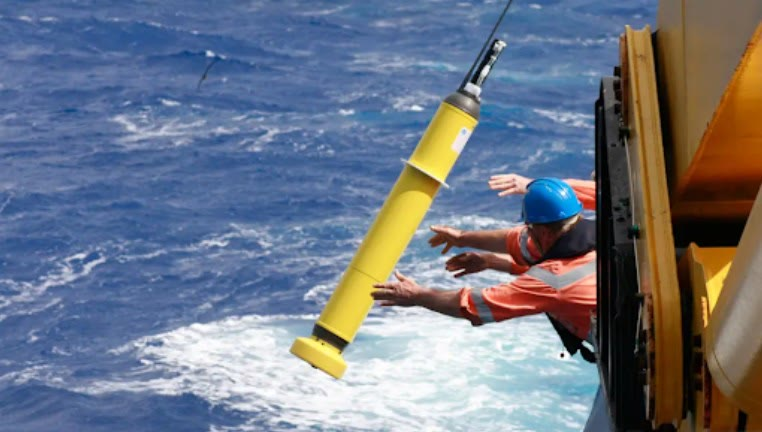
\includegraphics[width=\linewidth]{images/book5/b3-argo-deploy.jpg}

{\scriptsize Een Argo-drijver die over de zijkant van een onderzoeksschip wordt gelaten (NOAA
Global Ocean Monitoring and Observing Program, publiek domein).}
\end{minipage}
\end{inthefield}
% ledger: argo:fleet, noaa:argo-25, photo:b3-argo-deploy

\section{Oceaangetijden}\label{sec:b3:ocean-dynamics:tides}

Twee keer per dag, elke dag iets minder dan een uur later, stijgt en daalt de
zee. De natuurkundeboeken leggen de getijkracht uit: de aantrekking van de Maan is
op de nabije zijde van de Aarde sterker dan in het midden, en op de verre zijde
zwakker, zodat het water ten opzichte van het midden aan beide kanten langs de
lijn naar de Maan wordt uitgerekt.

\begin{definition}[Evenwichtsgetij; getijcomponent]\label{def:b3:ocean-dynamics:tides}
Het \emph{evenwichtsgetij}\index{evenwichtsgetij} is de vorm die het oppervlak van een oceaan
die de hele Aarde bedekt zou aannemen als het de getijdenpotentiaal
zonder traagheid onmiddellijk zou volgen. Een \emph{getijcomponent}\index{getijcomponent} is een van de
harmonische termen, elk met een vaste frequentie die door de bewegingen van de Maan
en de Zon wordt bepaald, en met een amplitude en fase die op elke plaats wordt gevonden,
en waarvan de som het getij vormt; ze worden aangeduid met een letter en het aantal
cycli per dag, zoals M$_2$, de
principale maansemidiurnale getijcomponent.
\end{definition}

\begin{theorem}[Evenwichtsgetij van de Maan]\label{thm:b3:ocean-dynamics:equilibrium-tide}
Voor de Maan, met massa $M$ op afstand $d$ van het middelpunt van de Aarde, met
massa $M_E$ en straal $a$, is het \omterm{def:b3:ocean-dynamics:tides}{evenwichtsgetij} onder een hoek $\theta$ van
het punt onder de Maan
\[
\eta = K\,\frac{3\cos^2\theta - 1}{2},\qquad
K = \frac{M}{M_E}\Big(\frac{a}{d}\Big)^3 a .
\]
\end{theorem}

\begin{proof}
De potentiaal van de Maan in een punt op afstand $a$ van het middelpunt van de
Aarde en onder hoek $\theta$ is $-GM/s$, met $s^2 = d^2 - 2ad\cos\theta +
a^2$. Ontwikkelen naar $a/d$ levert $1/s = (1/d)[1 + (a/d)\cos\theta + (a/d)^2
(3\cos^2\theta - 1)/2 + \cdots]$. De eerste term is een constante; de tweede
is een uniform veld, dat de hele Aarde in haar baan rond het gemeenschappelijke
massamiddelpunt versnelt, en heeft geen effect ten opzichte van de Aarde. Wat
overblijft is de getijdenpotentiaal $\Phi_T = -(GMa^2/d^3)(3
\cos^2\theta - 1)/2$. In evenwicht is het zeeoppervlak een oppervlak van
constante totale potentiaal, $g\eta + \Phi_T = C$, met $g = GM_E/a^2$, dus
$\eta = (M/M_E)(a^4/d^3)(3\cos^2\theta - 1)/2 + C/g$. Het gemiddelde van
$3\cos^2\theta - 1$ over de bol is nul; omdat het volume water
vaststaat, is $C = 0$.
\end{proof}

Met de massaverhouding $0.0123$, $d = \qty{384400}{km}$ en $a =
\qty{6371}{km}$ volgt $K = \qty{0.357}{m}$: de zee staat \qty{0.36}{m}
hoog onder de Maan en aan de tegenoverliggende kant, en \qty{0.18}{m} laag op
de grootcirkel daartussen, een spreiding van \qty{0.54}{m}. Op breedte $\varphi$,
met de Maan op declinatie $\delta$ en op uurhoek $H$, geldt $\cos\theta =
\sin\varphi\sin\delta + \cos\varphi\cos\delta\cos H$. Terwijl de Aarde
onder de twee bulten draait, passeert een plaats in een maandag twee hoogwaters,
\qty{24}{h} \qty{50}{min}: het halfdaagse getij. Wanneer de Maan
ten noorden of zuiden van de evenaar staat, zijn de twee bulten gekanteld, en de
twee hoogwaters van een dag zijn ongelijk, zoals de figuur hieronder laat zien. De Zon
veroorzaakt een getij van dezelfde vorm, \num{0.46} keer zo groot; de twee tellen op bij nieuwe
en volle maan, bij springtij, en heffen elkaar gedeeltelijk op bij de kwartieren.
% ledger: moon5:orbit, earth:Rmean, stewart:tide-equilibrium (computed in figdata/bachelor-3/tides.py)

\begin{omfigure}
\begin{tikzpicture}
\begin{groupplot}[group style={group size=2 by 1, horizontal sep=1.9cm},
  tick label style={font=\scriptsize}, label style={font=\small},
  legend style={font=\scriptsize, draw=none, fill=none}]
\nextgroupplot[width=0.40\linewidth, height=0.40\linewidth, axis equal image, hide axis,
  clip=false, xmin=-1.3, xmax=2.0, ymin=-1.25, ymax=1.25]
% computed in figdata/bachelor-3/tides.py
\addplot[fill=omThm!12, draw=omThm, thick] table[x=x, y=y] {figdata/out/bachelor-3-tides-bulge.dat};
\addplot[black, fill=black!10, domain=0:360, samples=91] ({cos(x)}, {sin(x)});
\draw[->, >=stealth, thick] (axis cs:1.25,0) -- (axis cs:1.95,0);
\node[above, font=\scriptsize, align=center] at (axis cs:1.6,0.08) {naar de\\Maan};
\node[font=\scriptsize] at (axis cs:0,0) {Aarde};
\nextgroupplot[width=0.54\linewidth, height=0.40\linewidth, xlabel={tijd (\unit{h})},
  ylabel={$\eta$ (\unit{m})}, xmin=0, xmax=49.6, xtick={0,12,24,36,48}, ymin=-0.2, ymax=0.4,
  legend style={at={(axis cs:12.4,0.39)}, anchor=north}, legend cell align=left, legend columns=2]
\addplot[omDef, thick] table[x=t, y=eta0] {figdata/out/bachelor-3-tides-series.dat};
\addlegendentry{$\delta = 0$}
\addplot[omThm, thick] table[x=t, y=eta20] {figdata/out/bachelor-3-tides-series.dat};
\addlegendentry{$\delta = \ang{20}$}
\addplot[black!50, thin, forget plot] coordinates {(0,0) (49.6,0)};
\end{groupplot}
\end{tikzpicture}

\par\smallskip{\small Links, het \omterm{def:b3:ocean-dynamics:tides}{evenwichtsgetij} van de Maan, in het vlak
dat de Maan bevat, de bult ongeveer twee miljoen keer overdreven. Rechts,
het \omterm{def:b3:ocean-dynamics:tides}{evenwichtsgetij} op \ang{45} NB over twee maandagen, met de
Maan op de evenaar (blauw) en op declinatie \ang{20} NB (rood): het tweede
geval heeft het ene hoogwater veel hoger dan het andere, de dagelijkse
ongelijkheid.}\label{fig:b3:ocean-dynamics:equilibrium-tide}
\end{omfigure}
% ledger: moon5:orbit, stewart:tide-constituents

De harmonische analyse van het \omterm{def:b3:ocean-dynamics:tides}{evenwichtsgetij} levert de componenten op. De
vijf grootste, met hun evenwichtsamplitudes, staan in de tabel hieronder. Ten
minste 39 componenten zijn nodig om het getij van een haven te voorspellen tot op een duizendste van
de grootste term, en een meetpunt moet langer dan 18.6 jaar lopen, de periode
van de modulatie van de maangetijden, om ze allemaal te scheiden.

\begin{center}
\small
\begin{tabular}{llrr}
\hline
component & oorsprong & periode (\unit{h}) & evenwichtsamplitude (\unit{m}) \\
\hline
M$_2$ & principaal maans, halfdaags & \num{12.4206} & \num{0.2423} \\
S$_2$ & principaal zonnes, halfdaags & \num{12.0000} & \num{0.1128} \\
N$_2$ & maans elliptisch, halfdaags & \num{12.6584} & \num{0.0464} \\
K$_1$ & lunisolair, daags & \num{23.9344} & \num{0.1416} \\
O$_1$ & principaal maans, daags & \num{25.8194} & \num{0.1005} \\
\hline
\end{tabular}
\end{center}
% ledger: stewart:tide-constituents, stewart:tide-prediction

Het werkelijke getij is niet het \omterm{def:b3:ocean-dynamics:tides}{evenwichtsgetij}. Om een bult onder de Maan
op de evenaar vast te houden, zou het getij in een maandag rond de Aarde moeten
lopen, met ongeveer \qty{460}{m/s}, een snelheid die een lange zwaartekrachtgolf
alleen bereikt in een oceaan van \qty{22}{km} diep; en de continenten
houden het tegen. Het getij is in plaats daarvan een gedwongen lange golf, die in elk bekken bijna in resonantie heen en weer klotst, en de
rotatie van de Aarde laat hem om het bekken draaien.
% ledger: stewart:tide-prediction

\begin{definition}[Kelvingolf]\label{def:b3:ocean-dynamics:kelvin-wave}
Een oceanische \emph{Kelvingolf}\index{Kelvingolf} is een lange zwaartekrachtgolf
die langs een kust, of langs de evenaar, loopt zonder snelheid dwars erop,
waarbij zijn hoogte exponentieel afneemt op afstand van de kust over de
Rossbystraal. Langs een kust loopt hij met de kust aan zijn rechterhand op het
Noordelijk Halfrond, aan zijn linkerhand op het Zuidelijk.
\end{definition}

\begin{theorem}[Kelvingolf aan de kust]\label{thm:b3:ocean-dynamics:kelvin}
In een oceaan met uniforme diepte $H$ op een $f$-vlak, met $f > 0$, begrensd door een
rechte kust langs $y = 0$ en gelegen in $y > 0$, geldt voor de lineaire
ondiepwatervergelijkingen dat ze oplossingen hebben met $v = 0$
\[
\eta = \mathrm e^{-y/L_R}F(x - ct),\qquad u = \frac{g}{c}\,\eta,\qquad
c = \sqrt{gH},\quad L_R = \frac{c}{f},
\]
voor elk willekeurig profiel $F$, en geen enkele oplossing met $v = 0$ loopt in de richting
$-x$.
\end{theorem}

\begin{proof}
Met $v = 0$ luiden de vergelijkingen $\partial u/\partial t = -g\,\partial\eta/
\partial x$, $fu = -g\,\partial\eta/\partial y$ en $\partial\eta/\partial t
+ H\,\partial u/\partial x = 0$. De eerste en de derde geven $\partial^2
\eta/\partial t^2 = gH\,\partial^2\eta/\partial x^2$: in $x$ draagt elke lijn
$y = $ constant golven $F(x \mp ct)$ met $c = \sqrt{gH}$, en dan geeft de
eerste vergelijking $u = \pm(g/c)\eta$. De tweede wordt $\partial\eta/
\partial y = \mp(f/c)\eta$, dus $\eta \propto \mathrm e^{\mp y/L_R}$. Met
het bovenste teken neemt de golf af op afstand van de kust; met het onderste
zou hij zonder grens de oceaan in groeien, wat wordt uitgesloten. De golf
gaat naar $+x$ met de oceaan aan zijn linkerhand, de kust aan zijn rechterhand.
\end{proof}

Over de diepe oceaan, \qty{4000}{m} diep, is $c = \qty{198}{m/s}$ en is de
Rossbystraal bij middelbrede breedten ongeveer \qty{2000}{km}: het getij loopt
rond een heel bekken. Boven een shelfzee van \qty{50}{m} diep is $c =
\qty{22}{m/s}$, ligt de Rossbystraal onder \qty{200}{km}, en is de
M$_2$-golflengte ongeveer \qty{1000}{km}. In een inham keert het getij dat langs
de ene kust als \omterm{def:b3:ocean-dynamics:kelvin-wave}{Kelvingolf} binnenkomt terug langs de tegenoverliggende kust,
opnieuw met de kust aan zijn rechterhand; de twee golven heffen elkaar op in punten daartussen.

\begin{definition}[Amfidromisch punt; cotidale lijn; corangelijn]\label{def:b3:ocean-dynamics:amphidrome}
Een \emph{amfidromisch punt}\index{amfidromisch punt} is een punt waar de
amplitude van een \omterm{def:b3:ocean-dynamics:tides}{getijcomponent} nul is en waaromheen het hoogwater
draait. Een \emph{cotidale lijn}\index{cotidale lijn} verbindt de plaatsen waar
het hoogwater van een component op hetzelfde moment valt; een \emph{corangelijn}\index{corangelijn}
verbindt de plaatsen met gelijke getijslag. Cotidale
lijnen stralen uit vanuit de amfidromische punten; corangelijnen cirkelen eromheen.
\end{definition}

\begin{omfigure}
\centering
\begin{tikzpicture}
\begin{axis}[width=0.96\linewidth, height=0.35\linewidth, axis equal image,
  xmin=0, xmax=1600, ymin=0, ymax=400, xtick={0,400,800,1200,1600}, ytick={0,200,400},
  xlabel={afstand langs het kanaal (\unit{km})}, ylabel={dwars (\unit{km})},
  tick label style={font=\scriptsize}, label style={font=\small}]
% computed in figdata/bachelor-3/tides.py
\addplot[omDef!70, densely dashed, unbounded coords=jump] table[x=x, y=y] {figdata/out/bachelor-3-tides-cor.dat};
\pgfplotsinvokeforeach{30,60,90,120,150,180,210,240,270,300,330}{
  \addplot[omThm, thin, unbounded coords=jump] table[x=x, y=y] {figdata/out/bachelor-3-tides-cot-#1.dat};
}
\addplot[omThm, very thick, unbounded coords=jump] table[x=x, y=y] {figdata/out/bachelor-3-tides-cot-0.dat};
\addplot[only marks, mark=*, mark size=2pt] table[x=x, y=y] {figdata/out/bachelor-3-tides-amph.dat};
\addplot[->, >=stealth, very thick, domain=20:310, samples=60] ({742.7+70*cos(x)}, {200+70*sin(x)});
\end{axis}
\end{tikzpicture}

\par\smallskip{\small Twee Kelvingolven van het M$_2$-getij in een verzonnen
kanaal van \qty{400}{km} breed en \qty{50}{m} diep op \ang{55} NB, de ene
naar het oosten langs de zuidelijke kust, de andere naar het westen langs de noordelijke kust.
Rood, de \omterm{def:b3:ocean-dynamics:amphidrome}{cotidale lijnen}, elke \ang{30} fase (ongeveer een uur), de dikke voor
hoogwater op het tijdstip van de oorsprong; blauw gestreept, de \omterm{def:b3:ocean-dynamics:amphidrome}{corangelijnen}, elke
vijfde van de amplitude van een golf aan zijn kust. De amfidromische punten
(stippen) liggen op de middellijn een halve golflengte,
\qty{495}{km} uit elkaar, en het hoogwater draait om hen tegen de klok in
(pijl).}\label{fig:b3:ocean-dynamics:amphidromes}
\end{omfigure}

De kaarten van het oceaangetij, gemaakt met satellietaltimetrie, nauwkeurig tot
ongeveer \qty{2}{cm} op de diepe zee, tonen deze structuur overal: de
M$_2$-kam draait tegen de klok in rond de amfidromen van de bekkens op het
Noordelijk Halfrond en met de klok mee op het Zuidelijk, en de grootste
getijslagen liggen aan de kusten. De getijden dissiperen \qty{3.75}{TW}, waarvan
\qty{3.5}{TW} in de oceaan: ongeveer twee derde van de M$_2$-energie op de
shelven en in ondiepe zeeën, en een derde via interne golven in de diepe
oceaan. Die energie verlengt de dag met ongeveer \qty{2.07}{ms} per eeuw en
duwt de Maan per jaar \qty{3.86}{cm} weg; en het deel dat in de diepe oceaan
verloren gaat, mengt het water, en levert zo een deel van de menging die in het
beeld van Stommel--Arons de diepzeecirculatie aandrijft.
% ledger: stewart:tide-prediction


\section{Oefeningen}

\begin{exercise}[$\star$]\label{exo:b3:ocean-dynamics:1}
Een westelijke windschuifspanning van \qty{0.12}{Pa} waait over de zee op \ang{40} NB
($\rho = \qty{1025}{kg/m^3}$, $\Omega = \qty{7.292115e-5}{rad/s}$).
Bereken het Ekmanvolumetransport per meter breedte en zijn richting,
en het transport over een doorsnede van \qty{1000}{km} lang, in sverdrup.
\end{exercise}

\begin{exercise}[$\star$]\label{exo:b3:ocean-dynamics:2}
Met $A_z = \qty{0.05}{m^2/s}$, bereken de \omterm{def:b3:ocean-dynamics:ekman-pumping}{Ekmandiepte} op \ang{45} NB. Welk
deel van de oppervlaktestroom blijft op die diepte over?
\end{exercise}

\begin{exercise}[$\star$]\label{exo:b3:ocean-dynamics:3}
Op \ang{30} NB is de krul van de windschuifspanning \qty{-1e-7}{Pa/m} over een
bekken van \qty{5000}{km} breed ($a = \qty{6371}{km}$). Bereken $\beta$, het
Sverdruptransport per eenheid van breedte en het totale transport, met zijn
richting.
\end{exercise}

\begin{exercise}[$\star$]\label{exo:b3:ocean-dynamics:4}
Bereken uit de perioden van M$_2$ en S$_2$ de periode van de cyclus van
springtij en doodtij, de tijd tussen twee uitlijningen van de twee
componenten.
\end{exercise}

\begin{exercise}[$\star\star$]\label{exo:b3:ocean-dynamics:5}
Een westelijke spanning neemt lineair toe van 0 bij \ang{35} NB tot \qty{0.1}{Pa} bij
\ang{45} NB, \qty{1110}{km} verder noordelijk. Bereken de \omterm{def:b3:ocean-dynamics:ekman-pumping}{Ekmanpompen} bij
\ang{40} NB, met behoud van beide termen van \cref{prop:b3:ocean-dynamics:pumping},
in meter per jaar. Wordt het water omhoog of omlaag geduwd?
\end{exercise}

\begin{exercise}[$\star\star$]\label{exo:b3:ocean-dynamics:6}
In een Stommelgyre met $r = \qty{2e-6}{s^{-1}}$ en $\beta =
\qty{2e-11}{m^{-1}.s^{-1}}$, bereken de breedte $\delta_S$. Als de randstroom
\qty{30}{\sverdrup} transporteert in de bovenste \qty{800}{m}, binnen een
breedte $\delta_S$, wat is dan zijn gemiddelde snelheid?
\end{exercise}

\begin{exercise}[$\star\star$]\label{exo:b3:ocean-dynamics:7}
Bereken de Munkbreedte $\delta_M$ en de breedte van de noordwaartse straalstroom,
$(2\pi/\sqrt3)\,\delta_M$, bij \ang{30} NB voor $A_H = \qty{e4}{m^2/s}$. Hoe
verandert de breedte als $A_H$ acht keer zo klein is?
\end{exercise}

\begin{exercise}[$\star\star$]\label{exo:b3:ocean-dynamics:8}
Twee stations \qty{80}{km} uit elkaar liggen op een lijn van west ($A$) naar oost
($B$) bij \ang{36} NB. Ten opzichte van het \qty{1000}{dbar}-oppervlak is de
geopotentiaalanomalie van het zeeoppervlak \qty{14.5}{J/kg} bij $A$ en
\qty{21.3}{J/kg} bij $B$. Bereken de oppervlaktestroom ten opzichte van
\qty{1000}{dbar} en de richting ervan. Welk station heeft de
warmere waterkolom?
\end{exercise}

\begin{exercise}[$\star\star$]\label{exo:b3:ocean-dynamics:9}
Met het \omterm{def:b3:ocean-dynamics:tides}{evenwichtsgetij} van de Maan, $K = \qty{0.357}{m}$, en de verhouding
\num{0.46} van het zonnegetij tot het maangetij, bereken de evenwichtsgetijslag
(hoogwater onder de hemellichamen min laagwater bij \ang{90}) bij springtij en bij
doodtij, en hun verhouding.
\end{exercise}

\begin{exercise}[$\star\star\star$]\label{exo:b3:ocean-dynamics:10}
Op het equatoriale $\beta$-vlak geldt $f = \beta_0y$ met $\beta_0 =
2\Omega/a$. Toon aan dat de \omterm{def:b3:ocean-dynamics:kelvin-wave}{Kelvingolf} $\eta = G(y)F(x - ct)$, $v = 0$,
overgaat in $G = \exp(-\beta_0y^2/2c)$, gevangen aan beide zijden van de evenaar,
en naar het oosten loopt. Bereken de invangschaal $\sqrt{c/\beta_0}$ voor een
golf met een snelheid van \qty{2.5}{m/s}.
\end{exercise}

\begin{exercise}[$\star\star\star$]\label{exo:b3:ocean-dynamics:11}
(a)~Leid $V = a\tan\varphi\,W_0$ af voor het abyssale binnenste uit $\beta v =
f\,\partial w/\partial z$. (b)~Bereken met $W_0 = \qty{e-7}{m/s}$ de $V$ bij
\ang{30} NB en het totale poolwaartse transport over een bekken van
\qty{5000}{km} breed. (c)~Waar moet het water vandaan komen?
\end{exercise}

\begin{exercise}[$\star\star\star$]\label{exo:b3:ocean-dynamics:12}
Een geostrofische stroom $W_g = u_g + \mathrm iv_g$ stroomt over een vlakke
zeebodem bij $z = 0$, met wervelviscositeit $A_z$ en geen slip op de bodem.
(a)~Toon aan dat $W = W_g(1 - \mathrm e^{-(1+\mathrm i)z/\delta})$, $\delta =
\sqrt{2A_z/f}$. (b)~Toon aan dat het transporttekort van deze bodem-Ekmanlaag
de verticale snelheid $w = \tfrac12\delta\zeta_g$ het binnenste in pompt, met
$\zeta_g$ de vorticiteit van de geostrofische stroom. (c)~Voor
$A_z = \qty{0.01}{m^2/s}$, $f = \qty{e-4}{s^{-1}}$ en een oceaan
\qty{4000}{m} diep, bereken $\delta$, de afremsnelheid $r =
f\delta/2H$, en de inverse daarvan in dagen.
\end{exercise}
% ledger: earth:Rmean, geod5:grs80-defining, stewart:tide-constituents, stewart:tide-equilibrium

\section{Probleem: Een gyre in de Zee van Ammar}

\begin{problem}[{Weekendprobleem --- Ekmanpompen, Sverdruptransport,
de westelijke randstroom en het getij van een verzonnen oceaan}]
\label{pb:b3:ocean-dynamics:1}
De Zee van Ammar is een verzonnen oceaanbekken, een rechthoek van \ang{20} tot
\ang{50} NB en \qty{6000}{km} breed, \qty{4000}{m} diep. De windschuifspanning is
zonaal, $\tau_x = -\tau_0\cos(\pi(\varphi - \ang{20})/\ang{30})$ met $\tau_0
= \qty{0.1}{Pa}$. Neem $\rho = \qty{1025}{kg/m^3}$, $\Omega =
\qty{7.292115e-5}{rad/s}$, $a = \qty{6371}{km}$, $g = \qty{9.81}{m/s^2}$,
en, waar een $\beta$-vlak gevraagd wordt, de waarde ervan bij \ang{35} NB.

\medskip\noindent\textbf{Deel I --- De Ekmanlaag.}
\begin{enumerate}
\item Bereken de windschuifspanning bij \ang{20}, \ang{35} en \ang{50} NB.
\item Bereken $f$ bij dezelfde breedtegraden.
\item Bereken het Ekman-volumetransport per eenheid van breedte bij \ang{20} en
  \ang{50} NB, met zijn richting. Convergeren of divergeren de transporten in
  het bekken?
\item Met $A_z = \qty{0.05}{m^2/s}$, bereken de \omterm{def:b3:ocean-dynamics:ekman-pumping}{Ekmandiepte} bij \ang{35} NB.
\item Bereken de \omterm{def:b3:ocean-dynamics:ekman-pumping}{Ekmanpompen} bij \ang{35} NB, in meter per seconde en per
  jaar.
\item Hoeveel jaar zou het duren voordat deze pomping het oppervlaktewater
  \qty{500}{m} omlaag heeft geduwd?
\end{enumerate}

\medskip\noindent\textbf{Deel II --- Het Sverdrup-binnenste.}
\begin{enumerate}[resume]
\item Bereken de lengte $L$ van het bekken van zuid naar noord en $\beta$ bij
  \ang{35} NB.
\item Bereken de krul van de windschuifspanning bij \ang{35} NB.
\item Bereken het Sverdruptransport per eenheid van breedte bij \ang{35} NB, met
  zijn richting.
\item Bereken het totale transport van het binnenste over het bekken bij
  \ang{35} NB, in sverdrups.
\item Als deze stroom zich over de bovenste \qty{1000}{m} verspreidt, wat is
  dan zijn gemiddelde snelheid, en hoeveel jaar doet een waterpakketje erover om
  \qty{1000}{km} naar het zuiden te bewegen?
\item Toon aan dat $fw_E/\beta$ bij \ang{35} NB hetzelfde transport geeft, en
  verklaar waarom met de \omterm{def:b3:atmospheric-dynamics:pv}{potentiële vorticiteit} van een kolom.
\end{enumerate}

\medskip\noindent\textbf{Deel III --- De westelijke randstroom.}
\begin{enumerate}[resume]
\item Verklaar waarom de terugstroom niet langs de oostkant van het bekken kan
  lopen.
\item Bereken met een bodemwrijving $r = \qty{e-6}{s^{-1}}$ de
  Stommelbreedte $\delta_S$.
\item Bereken het noordwaartse transport per eenheid van breedte aan de westelijke
  wand, $A(X/\delta_S - 1)$, en de gemiddelde snelheid als het de bovenste
  \qty{1000}{m} vult.
\item Hoe ver van de wand eindigt de noordwaartse stroom?
\item Bereken het noordwaartse transport van de Stommelgrenslaag, en verklaar
  waarom het ongeveer \qty{1.5}{\sverdrup} tekortschiet ten opzichte van het
  binnentransport.
\item Met $A_H = \qty{5e3}{m^2/s}$, bereken $\delta_M$ en de breedte van Munks
  noordwaartse straalstroom.
\item Munks straalstroom voert $1 + \mathrm e^{-\pi/\sqrt3}$ maal het
  binnentransport. Bereken het, en zeg waar het overschot naartoe gaat.
\end{enumerate}

\medskip\noindent\textbf{Deel IV --- Het getij van de Zee van Ammar.}
\begin{enumerate}[resume]
\item Bereken de snelheid van een \omterm{def:b3:ocean-dynamics:kelvin-wave}{Kelvingolf} in het bekken en de Rossbystraal
  bij \ang{35} NB.
\item Bereken de golflengte van de M$_2$-Kelvingolf.
\item Hoelang doet een \omterm{def:b3:ocean-dynamics:kelvin-wave}{Kelvingolf} erover om één keer rond de kusten van het
  bekken te lopen, en hoeveel M$_2$-perioden is dat?
\item Met welke snelheid zou het \omterm{def:b3:ocean-dynamics:tides}{evenwichtsgetij} over de cirkel van \ang{35} NB
  moeten lopen om onder de Maan te blijven, en in welke diepte van de oceaan zou
  een lange golf die snelheid halen?
\item Waar verwacht je het amfidromische punt van het bekken, en welke kant
  draait het hoogwater eromheen?
\item Bereken de halfdaagse evenwichtsamplitude bij \ang{35} NB, $\tfrac34
  K\cos^2\varphi$, met $K = \qty{0.357}{m}$, voor de Maan op de evenaar.
\item Geef het transport van de westelijke randstroom die de gyre van de Zee van
  Ammar sluit.
\end{enumerate}
\end{problem}
% ledger: earth:Rmean, geod5:grs80-defining, stewart:tide-constituents
